This dissertation shows ways to provide autonomous feedback for a range of assignment types in online computer science education. I believe that the ideas presented in this thesis are a step towards inclusive, quality education at scale.

\section{The Cause}

In September 2000, at the edge of the East River in New York City, the largest gathering of world leaders convened for the Millenial Summit. Bill Clinton, Daniel Moi, Mahathir Mohamad and 148 other heads of states came to represent their citizens. The aim of the summit leader, Kofi Annan, was to sieze the compelling symbolism of a unique moment in time to reflect on the sort of global future the leaders hoped for. At the meeting, the delegates came to the concensus that education is ``a foundation for human fulfilment, peace, sustainable development, economic
growth, decent work, gender equality and responsible global citizenship" (among other redeeming qualities) and as such should be one of the primary foci of the world stage. The delegates encoded their disiterata for the future into a set of twelve Millenium Development Goals to be achieved by December 2015. One of the goals was to attain universal primary education -- a reasonable first step. 

There are two months left until the Millenium Development Goals deadline. As such, it a particularly interesting point in time to reflect on where the world stands with respect to providing education. In the words of the United Nations, the education Millenium Development Goal of universal primary education will be ``unifinished." The global primary completion rate has reached 90\%\footnote{Net completion rate is the ratio of children of official school age who have completed a course to the population of the corresponding official school age. Secondary education completes the provision of basic education that began at the primary level, and aims at laying the foundations for lifelong learning and human development, by offering more subject- or skill-oriented instruction using more specialized teachers.} (according to the world bank) and the secondary and tertiary \emph{enrollment} rates are around 70\% and 30\% respectively. The most palpable meaning hidden behind these statistics is the sheer magnitude of human potential around the world that is being lost. Hundreds of millions of people don't have the opportunity to even enroll in secondary school. Looking even slightly deeper than this simple statistic further highlights the magnitude of the education challenge. Many who enroll don't complete, and completion does not mean that students are proficient with respect to the desired learning outcomes. Quality, it seems was an essential word left out of the initial goal. Moreover, the cost, born by both students, their families or governments relying on fickle internation aid, has been large. In the United States, Student debt is now \$1.2 trillion dollars and has surpassed consumer debt. The achievement gap between students of different S.E.S. groups is widening.

%The point of looking at education through the lense of the Millenium Development goals is two fold. First, it highlights that the need for education is a call that comes from the highest levels of government and the most basic human instincts. And second, it has been a driving force for measuring the staggering magnitude of the challenge. 

This year the Millenium Development Goals will be replaced by the United Nations Sustainable Development Goals. The new education objective is to, ``Ensure inclusive and quality education for all and promote lifelong learning." It includes subgoals for universal access to both primary and secondary education with expanded chanels for tertiary and adult education opporunities. The deadline to meet this goal is by 2030. To me this high bar makes sense. Lack of access to education is a great injustice and the sooner we address it, the sooner we can reap the rewards of a more equal world. But the magnitude of the new education challenge is titanic.

\section{The Feedback Challenge}

Online learning engenders hope that the constant interative improvement and economies of scale of the internet can help answer the question: How does high quality, inclusive, education scale? In 2012 Stanford, Harvard and MIT opened up access to the materials for some of the most prestigeous courses in the world for free. These Massive Open Online Courses (MOOCs) joined an ecosystem that had already shown the ability to tap into enormous demand. Khan Academy, whose mission is to provide, ``a free, world-class education for anyone, anywhere" was serving over 10 million monthly active users. The excitement was high and the New York Times declared the Year of the MOOC.

While new web technologies allow for scalable ways to deliver video lecture content,
implement social forums and track student progress in online courses, they remain limited in their ability to evaluate and give
feedback for complex and often open-ended student assignments such as programming assignments, mathematical proofs, design problems and
essays. 
This is not especially suprising given that providing feedback is one of the most time consuming parts of in person teaching \cite{sadler2006impact}. In courses where the student-teacher ratio can be ten thousand to one or worse, it is impossible for instructors to personally give hints to students or to understand the multitude of student approaches and pitfalls. As a result online courses are faced with a tradeoff. Either given rich beautiful assignments that can inspire students that have little to no feedback. Or, on the other hand give short answer questions and attempt to autonomously provide feedback in the limited domain. Both options are lacking. It is hard to imagine an education that doesn't involve engaging assignments and the scaffolding and feedback for those assignments that are a staple of the in-person classroom experience. Moreover, if feedback can be personalized and istantanous it can have benefits beyond those enjoyed in a conventional classroom. In his now famous work, the Two-Sigma Problem, Benjamin Bloom notes that on average students who are taught by a tutor with feedback-corrective procedures perform better that 98\% of students in conventional classroom \cite{corbett2001cognitive}. This gulf between what is currently possible and what
we think would improve open access learning suggests a research
challenge: Can we autonomously (or semi autonomously) generate feedback to rich assignments at scale?


Interestingly, an elegant solution to the high cost of giving feedback in massive classes is highlighted by the volume of student work. When thousands or even millions of students work on the same curriculum many higher level patterns take form. I have observed this structure on three different scales. 
\begin{enumerate}
\item There are shared substructures amongst student solutions (and partial solutions). Teachers observe this phenomena often while grading. Once you have seen a sufficient number of assignment submissions it often feels like you have seen everything. 
\item There are patterns in how students navigate the. When students work on an assignment from start to finish, the steps that they go through are not random and with enough students the contours of the assignment space emerge. 
\item There are curriculum level patterns between assignments. How students respond to earlier assignments has a strong impact on how they will respond to future assignments. With enough students these interdependencies can be measured.
\end{enumerate}
Collectively I refer to these three scales of patterns as Emergent Learner-Assignment Structure. I first enountered these patterns in prelimilary work on understanding students over time. Using a simple Markov Model of students working through introductory Computer Science courses, I found that there were prototypical patterns in \emph{how} students navigated their way to the final solution that could predict their exam scores more accurately than the students final assignment grade \cite{piech2012modeling}. 

\begin{mdframed}
My leading hypothesis in this book is that we can autonomously (or semi autonomously) generate feedback to rich assignments at scale by finding meaningful patterns in Emergent Learner-Assignment Structure. 
\end{mdframed}

If we are able to understand the patterns in Emergent Learner-Assignment Structure that enable autonomous feedback, we will have a solid foundation from which to generate new scientific understanding about the process of learning. While this is not the primary objective of my research, it is an important corollary.

Admittedly the space of all assignments is quite large. In this book, I ground my exploration into this challenge in the domain of Computer Science (CS) education. CS makes for a good case study. It is a prolific subject taught online, it is especially hard to learn without engaging in rich assignments and often (but not always) the assignments are programming tasks which have students create responses in a structured programming grammar.

\section{The Problem is Hard}

The task of modelling and predicting how human beings learn is informed by fields as diverse
as education, psychology, neuroscience and cognitive science. From a social science perspective
learning has been understood to be influenced by complex macro level interactions including affect
, motivation and even identity. The challenges present are further exposed on the micro
level. Learning is fundamentally a reflection of human cognition which is a highly complex process.
Two themes in the field of cognitive science that are particularly relevant are theories that the human
mind, and its learning process, are recursive and driven by analogy.

Nested milestones: Understand the space of partial solutions to an assignment.
->
Understand the path students take through partial solutions.
->
Understand student development across assignments. 
For domains which are more complex, we need to first focus on the most basic milestone. For domains which are simple, using techniques presented in this thesis, we can show notable gains on the 

Moreover, though unit tests are a useful way to test if final solutions are correct they are not well suited for giving help to students with an intermediate solution and they are not able to give feedback on stylistic elements.


%jobs vs graduates



%\section{Stolen Wording from Other Papers}

%Computer-assisted education promises open access to world class instruction and a reduction in the growing cost of learning.
%We can develop on this promise by building models of large scale student trace data on popular educational platforms such as Khan Academy, Coursera, and EdX. 

%We leverage the redundancy of densely sampled, highly structured homeworks in order 
%to force-multiply teacher effort. Giving articulate, instant feedback is a crucial component of the online learning process 
%and thus by building a homework search engine we hope to take a step towards higher quality free education.

%In the last few years, MOOCs have begun offering educational opportunities at zero cost to anyone with an internet connection~\cite{pappano12}.
%People of all ages from all over the world are increasingly turning to online resources to learn,
%and as a result, the sheer amount of data collected about student learning has grown astronomically, eclipsing previous records.
%The growth of free access education and the increasing demand for higher education, especially in Science, Technology, Engineering and Math, motivates the need, more than ever, to organize the enormous amount of collected student data
%in an intelligent way so that we can search the data and find patterns in order to benefit both students and instructors. 



%\section{The Contemporary Challenge}

%Massive open online courses (MOOCs), one of the latest internet revolutions have engendered hope that constant iterative improvement and economies of scale may cure the ``cost disease" of higher education. 
%While scalable in many ways, providing feedback for homework submissions (particularly open-ended ones) remains a challenge in the online classroom.  
%In courses where the student-teacher ratio can be ten thousand to one or worse, it is impossible for instructors to personally give feedback to students or to understand the multitude of student approaches and pitfalls. Organizing and making sense of massive collections of homework solutions is thus a critical web problem. Despite the challenges, the dense solution space sampling in highly structured homeworks for some MOOCs suggests an elegant solution to providing quality feedback to students on a massive scale. 

%In massive online courses that have thousands and sometimes millions of students it is often unfeasible to provide feedback on assignments of any complexity \cite{pappano2012year}.  As a result simple multiple choice questions, not open ended assessments, are the staple of online learning. The inability to provide feedback even applies to richly-structured assignments (such as math proofs or computer programs) where students create responses in a highly expressive, formalized grammar. Beautiful assessments can inspire students and add artistry to a course. This gulf between what is currently possible and what we think would improve open access learning suggests a research challenge: imagine and evaluate ways to give feedback to richly-structured assessments at scale. We believe that data of how previous students
%navigated their way to a final answer can
%be leveraged to autonomously understand the landscape of such assessments and enable hints for future students.

%Domain: Computer Science Education

Online computer science courses can be massive
with numbers ranging from thousands to even millions of students.
Though technology has increased our ability to provide 
content
to students at scale, assessing and providing feedback 
(both for final work and partial solutions) remains difficult.
Currently, giving personalized feedback, a staple of quality education, is costly for small, in-person classrooms and prohibitively expensive for massive classes. 
Autonomously providing feedback is therefore 
a central challenge for at scale computer science education.






Maybe we should hire more teachers? And we should support them better.

The sheer magnitude of lost opportunity creates a fierce urgency to the need for creative solutions.

For me the gap in opportunity is especially palpable. I grew up in Kenya going to International Schools until attending Stanford. The level of education my neighbors could expect to achieve is incomprable.

Massive open online courses (MOOCs) are the most recent
and highly publicized entrant to a rapidly expanding
universe of open educational resources.
In 2012 when Coursera first launched and the New York Times declared it the \"Year of the MOOC\" there was much excitement. However MOOCs, in their contemporary form, did not provide the pancea desired. They managed to scale the delivery of information without scaling the discussion sections, office hours, late-night dorm-room study groups, drop-in tutoring, painstakingly graded homework and other components of a successful large college class. 

\section{A Vision for the Future}
Autonomous feedback from a system that understands learners as they navigate complex learning environments.
In the far future, we may have powerful autonomous tutors. They will be able to understand what humans know and help them achieve learning goals in optimal ways. They will be free, or close to free. Their experience will persist. 

The core emphasis is two solve two problems (1) Provide feedback, (2) Select appropraite material for students. 

Achieving these milestones often involve sub-goals such as being able to predict what students will do, or how teachers would respond.

The autonomous feedback engine must be easy to author so that new activities and inspired ideas can be incorporated without much friction.

There are many different paths to an improved education landscape. This is just one interesting avenue.

One reason that online is interesting is that it may enable scientific insights into learning

Disiterata:
Easy to author.
Handle Richly Structured Activities

Teachers have historically been faced with a difficult decision on how much personalized
feedback to provide students on open-ended homework submissions
such as mathematical proofs, computer programs or essays. On one hand, feedback
is a cornerstone of the educational experience which enables students to
learn from their mistakes. On the other hand, giving comments to each student
can be an overwhelming time commitment. Hopefully autonomous feedback can be a powerful tool to help teachers of the future.


\section{Unique Access to Data}

Interestingly, a potential solution to the high cost of giving feedback in
massive classes is highlighted by the volume of student work.  Moreover data of how previous students navigated their way to a
final answer can be leveraged to autonomously understand the landscape of
such assessments and enable hints for future students.

To explore feedback at scale I analyzed some large, novel, educational
datasets. I amalgamated data from Coursera, Khan Academy, Code.org (which is to the
best of my knowledge the largest online course to date) and Stanford University.
See table \ref{tab:dataTable} for details. The research I have done often has immediate and clear
potential for social benefit.

\begin{table}[t]
 \centering
 \ra{1.3}
 \begin{tabular}{lp{1.8cm}p{1.8cm}p{1.8cm}p{1.8cm}p{1.8cm}}
   \toprule

   \tabhead{Statistic} & \tabhead{Khan \linebreak Geometry} & \tabhead{Code.org Academy} & \tabhead{Stanford CS106A} &  \tabhead{Coursera M.L.} & \tabhead{Coursera H.C.I.} \\

   \midrule

   Students & 1.0 $M$ & 1.2 $M$ & 2.7 $K$ & 26.1 $K$ & 7.2 $K$ \\
   Assignments  & 69 & 20 & 5 & 8 & 10 \\
   Submissions & 14.4 $M$ & 22.8 $M$ & 312.0 $K$ &  1.0 $M$  & 14.1 $K$ \\
   Type & Short & Programs & Programs & Programs & Report \\
   
   Temporal & Yes & Yes & Yes & No & No \\

   \bottomrule
 \end{tabular}
 \caption[Summary of datasets]{Summary of datasets analyzed. $K = $ thousands and $M = $ millions. M.L. = Machine Learning and H.C.I = Human Computer Interaction }
 \label{tab:dataTable}
\end{table}

In analyzing student learning in introductory programming
courses, there is a wealth of information not only in the final
products (i.e., programs) that students submit for evaluation, but
also in the development path they took to produce their programs.
In traditional settings, the data on how students developed their
programs over time is either not available or not analyzed. In this
work, we show that temporal traces of the development paths
taken by students in an introductory programming class can be
mined to build graphical models that compactly capture the
common major milestones in such development paths. More
significantly, we show that these models also carry predictive
capability in that the paths students take in these models are
correlated with their future performance in the class.

Richness of assignments has a very high spearman correlation with the sparcity of the solution space: the probability that a randomly sampled intermediate solution is unseen. I assume that the sparcity measure is generally independent of dataset size (after a certain point) because the data we observe tends to follow Zipfs law distributions. A general rule of thumb that I follow is that 

\begin{align}
richness &\sim log(p_{unseen}) \\
         &\sim log(u/n)
\end{align}

\section{Approaches}

\begin{figure}
\center
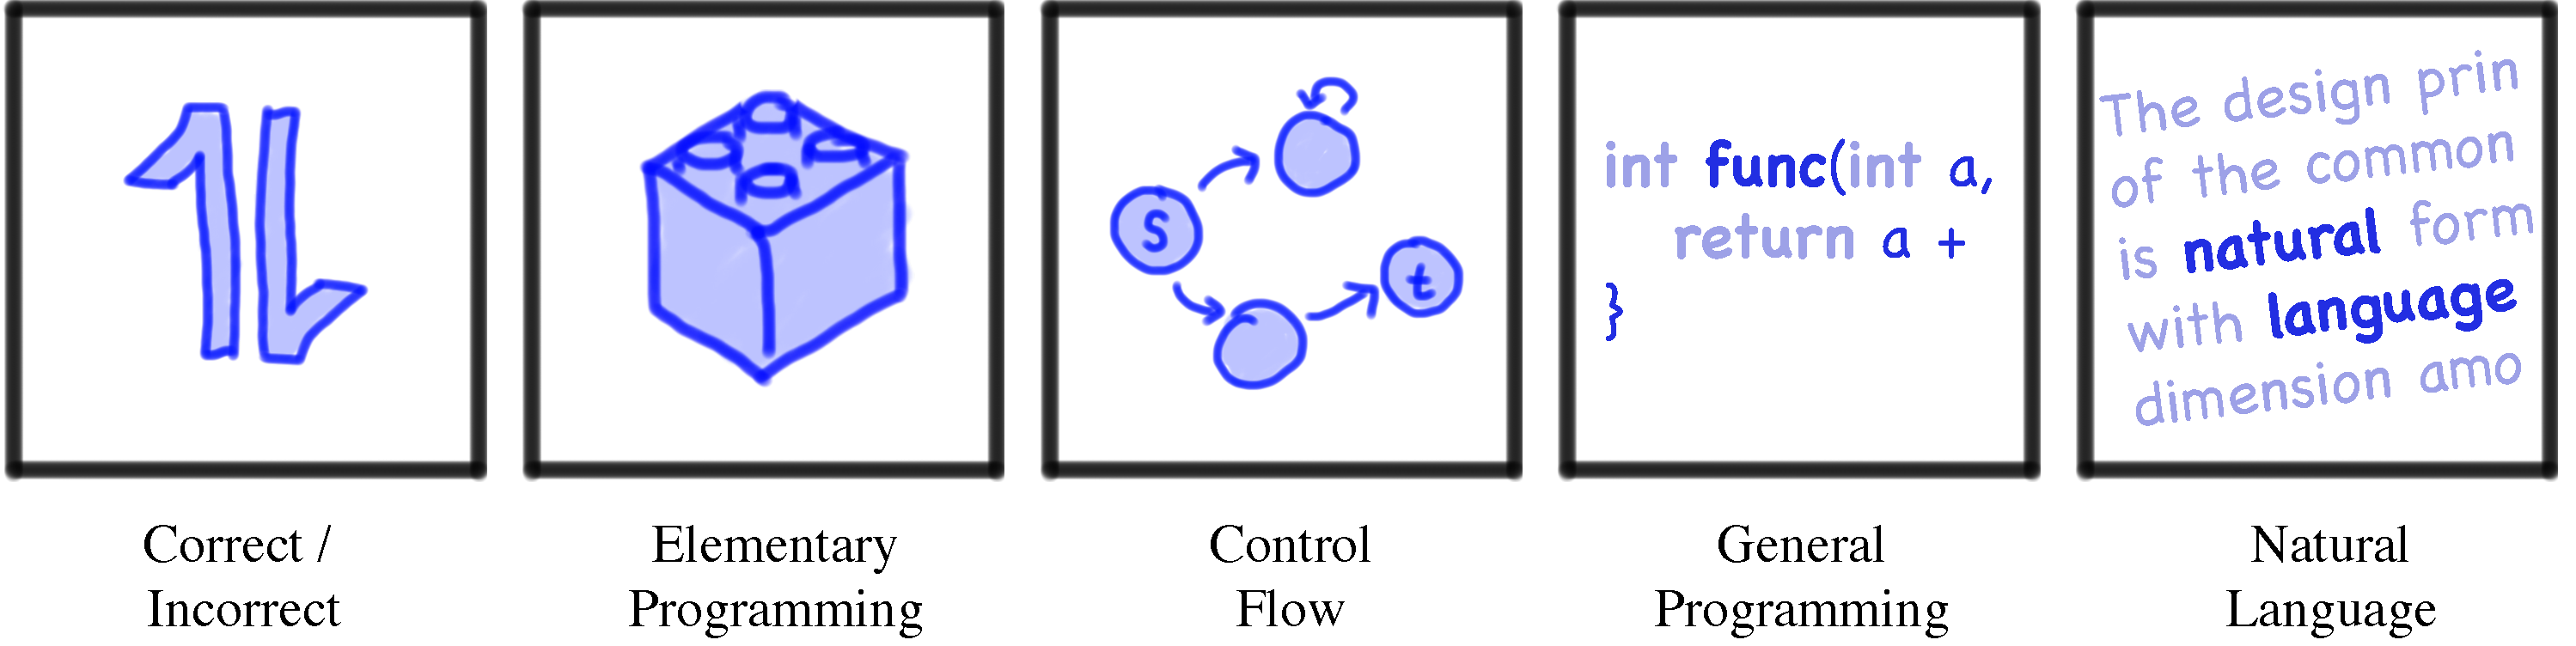
\includegraphics[width=1.0\textwidth]{img/assnType_all}
\caption{
The different types of assignments covered in this book.
}
\end{figure}

Neural networks. Try to first pose a testable machine learning task. \cite{piech2012modeling}

Find patterns in the corpus of student work. Find patterns in how students traverse the material. Generally for more simple assignments we are able to use temporal information, which is a very rich source of information. For the more complex assignments we need another approach.

Some interesting things to try a

Very unsupervised!

\section{Novel Contribution}

\begin{figure*}[t!]
\center
\subfigure[]{
   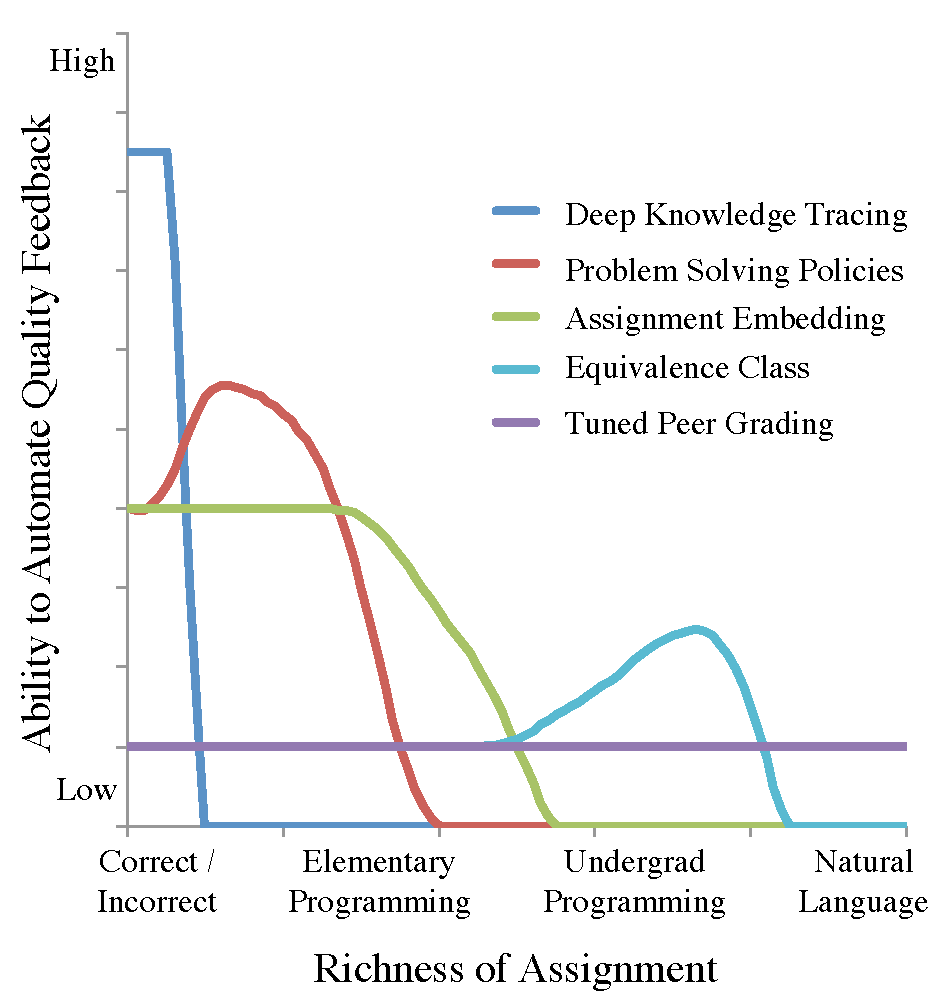
\includegraphics[width=.45\textwidth]{img/intro-projects.pdf}
   \label{fig:introProjects}
}
\subfigure[]{
   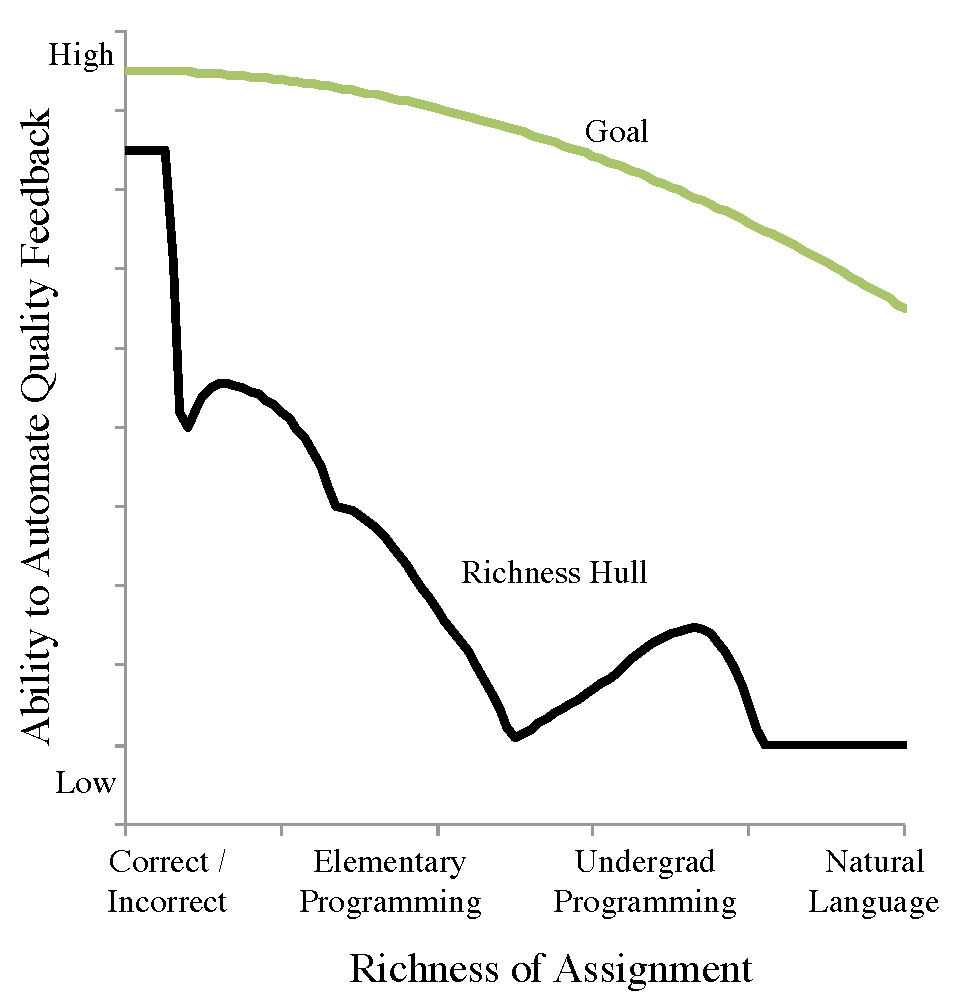
\includegraphics[width=.45\textwidth]{img/intro-impact.pdf}
   \label{fig:introImpact}
}

\caption{
\subref{fig:introProjects} What I did.
\subref{fig:introImpact} How it fits in with previous research.
}
\end{figure*}



State of the art in knowledge tracing

A novel way to \'tune\' the network of peer grades to simultaneously learn grading ability and assignment true scores

Contemporary autonomous tutors generally trace student knowledge as they solve simple correct or incorrect questions.


In this book:
Deep Knowledge Tracing
Crowd source students?
Finding Shared Substructure (programs)
Problem Solving Policies (programs)
Homework Embedding Spaces (programs)



Exploration of the space of feedback for richly structured assignments

\section{Ideas for the Future}

In this work we present a set of approaches that are appropriate for different types of assignments. Ideally in the future we will be able to achieve the level of autonomous feedback we see for khan data for more complex assignments. 

http://data.worldbank.org/indicator/SE.ENR.TERT.FM.ZS/countries/1W?display=graph